% questions.tex —— 1977 年·湖南株洲卷 · 题目内容片段（无答案）
% 由 tools/generate_projects.py 依来源总账自 1977/1977_数学真题_湖南株洲_试题.md 生成，勿手改（改源 MD 后重跑）


\gkpart{湖南省株洲（试点）}

\begin{gktip}
\textbf{来源说明}：本题面依据固定源 PDF《1977湖南株洲.pdf》第 1—10 页逐题转录。源卷是题面与解答连续排印的「试题解」型扫描件（页面底部带书籍页码 123—131），每题题面下紧接源印「解」或「证明」；正式题为第 1—15 题，第 9 题含（1）（2）两小问、分值随小问标注；末尾「参考题」3 道（原卷注明不记分、作完正题后有时间者可作），不计入题量。原卷未标注文理科。
\end{gktip}

\par\medskip

\begin{question}
\gkti{1}\textbf{（4 分）} $y=2\sqrt{x^2}$ 和 $y=2x$ 是不是同一个函数？为什么？

\end{question}
\begin{question}
\gkti{2}\textbf{（4 分）} 确定下列各式的符号：

（1） $1-\sin800^\circ$；

（2） $\cos20^\circ-\sin20^\circ$；

（3） $\operatorname{tg}288^\circ\cdot\operatorname{tg}510^\circ$。

\end{question}
\begin{question}
\gkti{3}\textbf{（4 分）} 已知 $x$、$y$ 都是实数，且 $(2x-1)^2+(y-8)^2=0$，求 $\log_2xy=\ \text{？}$

\end{question}
\begin{question}
\gkti{4}\textbf{（4 分）} $\sqrt{(\log_320)^2-6\log_320+9}=\ \text{？}$

\end{question}
\begin{question}
\gkti{5}\textbf{（6 分）} 已知 $\log_{15}7=a$，$\log_{15}8=b$，求 $\log_{56}15=\ \text{？}$

\end{question}
\begin{question}
\gkti{6}\textbf{（6 分）} 化简：

\nopagebreak[4]
\[
\left(\frac{x^{-1}-1}{x^{-1}+1}-\frac{x^{-1}+1}{x^{-1}-1}\right)\cdot\left(2^{-1}-4^{-1}x^{-1}-4^{-1}x\right).
\]

\end{question}
\begin{question}
\gkti{7}\textbf{（6 分）} $h$ 为什么数时，方程 $2hx^2+(8h+1)x=-8h$ 有两个不相等的实根？

\end{question}
\begin{question}
\gkti{8}\textbf{（6 分）} 证明恒等式：

\nopagebreak[4]
\[
\frac{2\sin\theta\cdot\sin\left(\dfrac{\pi}{2}-\theta\right)+\sin\left(\dfrac{3\pi}{2}+\theta\right)}
{1+\sin(\pi+\theta)+\sin^2(\pi-\theta)-\sin^2\left(\dfrac{\pi}{2}+\theta\right)}
=\operatorname{tg}\left(\dfrac{\pi}{2}-\theta\right).
\]

\Needspace{0.4\textheight}
\end{question}
\begin{question}
\gkti{9}

（1） （6 分） 三个半径都是 $R$ 的圆两两外切，求过三个切点的三个圆弧所围成图形的面积。

\begin{gktip}
原源 PDF 第 4 页附有三圆两两外切、圆心三角形与中间曲边区域示意图；LaTeX 版按源图重绘。
\end{gktip}
\nopagebreak[4]
\begin{center}% 1977 年湖南株洲卷第 9（1）题：三个半径都是 R 的圆两两外切；圆心三角形 ABC（等边），
% 切点 D 在 AB 上、F 在 AC 上、E 在 BC 上，中间曲边三角形加阴影（按源卷第 4 页布局）
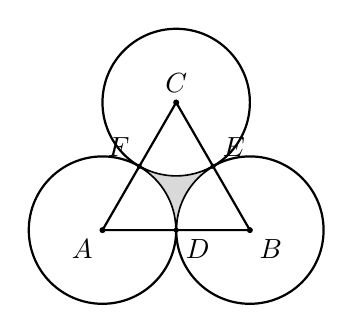
\begin{tikzpicture}[scale=0.78]
  \coordinate (A) at (0,0);
  \coordinate (B) at (2.4,0);
  \coordinate (C) at (1.2,2.078);
  \draw[thick] (A)--(B)--(C)--cycle;
  \draw[thick] (A) circle (1.2);
  \draw[thick] (B) circle (1.2);
  \draw[thick] (C) circle (1.2);
  \filldraw[fill=black!15] (1.2,0) arc (0:60:1.2) arc (240:300:1.2) arc (120:180:1.2) -- cycle;
  \fill (A) circle (1.4pt) node[below left] {$A$};
  \fill (B) circle (1.4pt) node[below right] {$B$};
  \fill (C) circle (1.4pt) node[above] {$C$};
  \fill (1.2,0) circle (1.2pt) node[below right] {$D$};
  \fill (0.6,1.039) circle (1.2pt) node[above left] {$F$};
  \fill (1.8,1.039) circle (1.2pt) node[above right] {$E$};
\end{tikzpicture}
\end{center}
\nopagebreak[4]
（2） （4 分） 已知菱形面积为 $392\ \mathrm{cm^2}$，有一角为 $150^\circ$，求边长。

\begin{gktip}
原源 PDF 第 4 页附有菱形与对角线示意图；LaTeX 版按源图重绘。
\end{gktip}
\nopagebreak[4]
\begin{center}% 1977 年湖南株洲卷第 9（2）题：菱形 ABCD（A 左、D 上、C 右、B 下），
% 对角线 BD 画虚线，A 处标 30°、B 处标 150°（按源卷第 4 页布局）
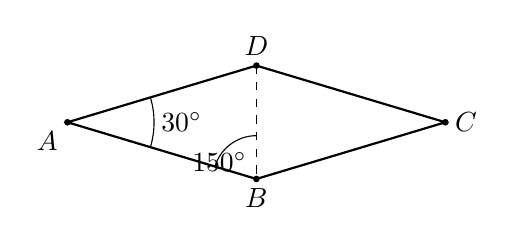
\begin{tikzpicture}[scale=1.0]
  \coordinate (A) at (0,0);
  \coordinate (D) at (2.4,0.72);
  \coordinate (C) at (4.8,0);
  \coordinate (B) at (2.4,-0.72);
  \draw[thick] (A)--(D)--(C)--(B)--cycle;
  \draw[dashed] (D)--(B);
  \draw ([shift=(16.7:1.1)]A) arc (16.7:-16.7:1.1);
  \node at (1.45,0) {$30^\circ$};
  \draw ([shift=(90:0.55)]B) arc (90:163.3:0.55);
  \node at (1.93,-0.50) {$150^\circ$};
  \fill (A) circle (1.2pt) node[below left] {$A$};
  \fill (B) circle (1.2pt) node[below] {$B$};
  \fill (C) circle (1.2pt) node[right] {$C$};
  \fill (D) circle (1.2pt) node[above] {$D$};
\end{tikzpicture}
\end{center}
\nopagebreak[4]
\Needspace{0.4\textheight}
\end{question}
\begin{question}
\gkti{10}\textbf{（6 分）} 在高 $150\ \mathrm{m}$ 的山顶上测得正南两船的俯角分别为 $15^\circ$ 和 $75^\circ$，求两船的距离。

\begin{gktip}
原源 PDF 第 5 页附有山顶俯角与两船位置示意图；LaTeX 版按源图重绘。
\end{gktip}
\nopagebreak[4]
\begin{center}% 1977 年湖南株洲卷第 10 题：山顶 P 处测正南两船 A、B 的俯角 15° 与 75°，
% PC 铅垂高 150m，DP 为过 P 的水平线（虚线），PA、PB 为视线（虚线）（按源卷第 5 页布局）
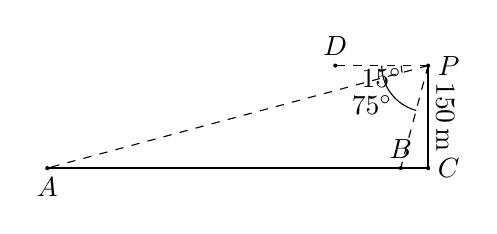
\begin{tikzpicture}[scale=0.62]
  \coordinate (P) at (0,0);
  \coordinate (D) at (-1.9,0);
  \coordinate (C) at (0,-2.1);
  \coordinate (B) at (-0.56,-2.1);
  \coordinate (A) at (-7.8,-2.1);
  \draw[thick] (A)--(C);
  \draw[thick] (C)--(P);
  \draw[dashed] (P)--(D);
  \draw[dashed] (P)--(A);
  \draw[dashed] (P)--(B);
  \draw ([shift=(180:0.55)]P) arc (180:195.2:0.55);
  \draw ([shift=(180:0.95)]P) arc (180:255.2:0.95);
  \node at (-0.95,-0.25) {$15^\circ$};
  \node at (-1.15,-0.80) {$75^\circ$};
  \fill (P) circle (1.2pt) node[right] {$P$};
  \fill (D) circle (1.2pt) node[above] {$D$};
  \fill (A) circle (1.2pt) node[below] {$A$};
  \fill (B) circle (1.2pt) node[above] {$B$};
  \fill (C) circle (1.2pt) node[right] {$C$};
  \node[rotate=-90] at (0.35,-1.05) {$150\,\mathrm{m}$};
\end{tikzpicture}
\end{center}
\nopagebreak[4]
\end{question}
\begin{question}
\gkti{11}\textbf{（8 分）} 有某种农药一桶，倒出 $8$ 升后，用水补满；然后又倒出 $4$ 升，再用水补满。于是测得桶中农药与水之比为 $18:7$，木桶的容积。

\begin{gktip}
\textbf{源注}：原卷题面末句印作「……之比为 $18:7$，木桶的容积。」，「木桶的容积」前无「求」字，系排印脱字；按语义应为求木桶的容积，转录保留原样。
\end{gktip}

\Needspace{0.4\textheight}
\end{question}
\begin{question}
\gkti{12}\textbf{（9 分）} 甲船在 $A$ 点发现乙船在北偏东 $60^\circ$ 的 $B$ 处，乙船以每小时 $a$ 浬的速度向北行驶，已知甲船速度是每小时 $\sqrt3\,a$ 浬，问甲船应依什么方向前进，才能最快地与乙船相会？

\begin{gktip}
原源 PDF 第 6 页附有航向角与追及示意图；LaTeX 版按源图重绘。
\end{gktip}
\nopagebreak[4]
\begin{center}% 1977 年湖南株洲卷第 12 题：甲船在 A 发现乙船在北偏东 60° 的 B 处，乙船北行，
% 甲船沿 AC 追及，相遇于 C；AN 指北，∠NAB=60°（按源卷第 6 页布局）
\begin{tikzpicture}[scale=0.58]
  \coordinate (A) at (0,0);
  \coordinate (B) at (2.6,1.5);
  \coordinate (C) at (2.6,4.5);
  \draw[->] (0,0)--(0,2.8);
  \node[above] at (0,2.8) {北};
  \node[left] at (0,2.1) {$N$};
  \draw[thick] (A)--(C);
  \draw[thick] (A)--(B);
  \draw[thick] (B)--(C);
  \draw ([shift=(90:1.0)]A) arc (90:30:1.0);
  \node at (0.78,0.85) {$60^\circ$};
  \fill (A) circle (1.2pt) node[below left] {$A$};
  \fill (B) circle (1.2pt) node[right] {$B$};
  \fill (C) circle (1.2pt) node[above right] {$C$};
\end{tikzpicture}
\end{center}
\nopagebreak[4]
\Needspace{0.4\textheight}
\end{question}
\begin{question}
\gkti{13}\textbf{（9 分）} 双曲线中心在原点，焦点在坐标轴上，焦距为 $14$，顶点间距离为 $12$，求双曲线方程。

\begin{gktip}
原源 PDF 第 7 页附有焦点在 $x$ 轴上与焦点在 $y$ 轴上的双曲线示意图各一幅；LaTeX 版按源图重绘。
\end{gktip}
\nopagebreak[4]
\begin{center}% 1977 年湖南株洲卷第 13 题图一：焦点在 x 轴上的双曲线 x^2/36 − y^2/13 = 1，
% 顶点 A(6,0)、A'(-6,0)，焦点 F2(7,0)、F1(-7,0)，B、B' 在 y 轴上 ±√13 处（按源卷第 7 页布局）
\begin{tikzpicture}[scale=0.44]
  \draw[->] (-8.6,0)--(8.6,0) node[below] {$x$};
  \draw[->] (0,-5.0)--(0,5.0) node[right] {$y$};
  \draw[thick] plot[domain=6:8.4,samples=30] (\x,{0.601*sqrt(\x*\x-36)});
  \draw[thick] plot[domain=6:8.4,samples=30] (\x,{-0.601*sqrt(\x*\x-36)});
  \draw[thick] plot[domain=-8.4:-6,samples=30] (\x,{0.601*sqrt(\x*\x-36)});
  \draw[thick] plot[domain=-8.4:-6,samples=30] (\x,{-0.601*sqrt(\x*\x-36)});
  \fill (6,0) circle (1.4pt) node[below right] {$A(6,0)$};
  \fill (-6,0) circle (1.4pt) node[below] {$A'$};
  \fill (7,0) circle (1.4pt) node[above] {$F_2\,(7,0)$};
  \fill (-7,0) circle (1.4pt) node[above] {$F_1$};
  \fill (0,3.606) circle (1.4pt) node[right] {$B$};
  \fill (0,-3.606) circle (1.4pt) node[right] {$B'$};
  \node[below left] at (0,0) {$O$};
\end{tikzpicture}
\end{center}
\nopagebreak[4]
\nopagebreak[4]
\begin{center}% 1977 年湖南株洲卷第 13 题图二：焦点在 y 轴上的双曲线 y^2/36 − x^2/13 = 1，
% 顶点 B(0,6)、B'(0,-6)，焦点 F(0,7)、F1(0,-7)，A、A' 在 x 轴上 ±√13 处（按源卷第 7 页布局）
\begin{tikzpicture}[scale=0.44]
  \draw[->] (-4.6,0)--(4.6,0) node[below] {$x$};
  \draw[->] (0,-9.4)--(0,9.4) node[right] {$y$};
  \draw[thick] plot[domain=6:9.2,samples=30] ({0.601*sqrt(\x*\x-36)},{\x});
  \draw[thick] plot[domain=6:9.2,samples=30] ({-0.601*sqrt(\x*\x-36)},{\x});
  \draw[thick] plot[domain=-9.2:-6,samples=30] ({0.601*sqrt(\x*\x-36)},{\x});
  \draw[thick] plot[domain=-9.2:-6,samples=30] ({-0.601*sqrt(\x*\x-36)},{\x});
  \fill (0,6) circle (1.4pt) node[right] {$B$};
  \fill (0,-6) circle (1.4pt) node[right] {$B'$};
  \fill (0,7) circle (1.4pt) node[right] {$F$};
  \fill (0,-7) circle (1.4pt) node[right] {$F_1$};
  \fill (3.606,0) circle (1.4pt) node[right] {$A$};
  \fill (-3.606,0) circle (1.4pt) node[left] {$A'$};
  \node[above left] at (0,0) {$O$};
\end{tikzpicture}
\end{center}
\nopagebreak[4]
\Needspace{0.4\textheight}
\end{question}
\begin{question}
\gkti{14}\textbf{（9 分）} 从等腰 $\triangle ABC$ 的顶点 $A$ 引直线交 $BC$ 于 $D$，交外接圆于 $E$，求证 $AB$ 是 $AD$ 和 $AE$ 的比例中项。

\begin{gktip}
原源 PDF 第 7 页附有等腰三角形外接圆与割线示意图；LaTeX 版按源图重绘。
\end{gktip}
\nopagebreak[4]
\begin{center}% 1977 年湖南株洲卷第 14 题：等腰△ABC 内接于圆，A 为顶点，割线 A-D-E 交 BC 于 D、
% 交外接圆于 E，BE 连虚线（按源卷第 7 页布局）
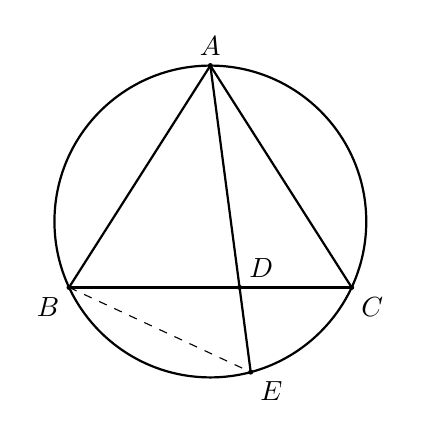
\begin{tikzpicture}[scale=0.66]
  \draw[thick] (0,0) circle (3);
  \coordinate (A) at (90:3);
  \coordinate (B) at (205:3);
  \coordinate (C) at (335:3);
  \coordinate (E) at (285:3);
  \coordinate (D) at (0.561,-1.268);
  \draw[thick] (A)--(B);
  \draw[thick] (A)--(C);
  \draw[thick] (B)--(C);
  \draw[thick] (A)--(E);
  \draw[dashed] (B)--(E);
  \fill (A) circle (1.4pt) node[above] {$A$};
  \fill (B) circle (1.4pt) node[below left] {$B$};
  \fill (C) circle (1.4pt) node[below right] {$C$};
  \fill (D) circle (1.4pt) node[above right] {$D$};
  \fill (E) circle (1.4pt) node[below right] {$E$};
\end{tikzpicture}
\end{center}
\nopagebreak[4]
\Needspace{0.4\textheight}
\end{question}
\begin{question}
\gkti{15}\textbf{（9 分）} 如果一个直角三角形三边的长成等差数列，试证明三边的比是 $3:4:5$。

\begin{gktip}
原源 PDF 第 8 页附有直角三角形三边示意图；LaTeX 版按源图重绘。
\end{gktip}
\nopagebreak[4]
\begin{center}% 1977 年湖南株洲卷第 15 题：直角三角形三边 a、a−d、a+d（按源卷第 8 页布局）
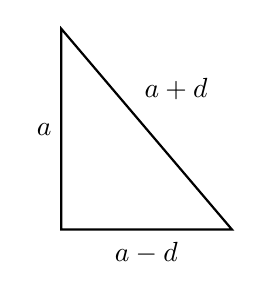
\begin{tikzpicture}[scale=0.85]
  \coordinate (T) at (0,3.0);
  \coordinate (L) at (0,0);
  \coordinate (R) at (2.55,0);
  \draw[thick] (T)--(L)--(R)--cycle;
  \node[left] at (0,1.5) {$a$};
  \node[below] at (1.27,-0.05) {$a-d$};
  \node[above right] at (1.1,1.8) {$a+d$};
\end{tikzpicture}
\end{center}
\nopagebreak[4]
\begin{gktip}
\textbf{参考题}（不记分、作完正题后，有时间者可作。）
\end{gktip}

\textbf{参考题 1．} 试求 $f(x)=x^4-42x^3+435x^2+113x-66$ 和 $g(x)=x^2-x-462$ 的公根。

\textbf{参考题 2．} 求函数 $y=\left(2x+1\right)^{\frac12}\left(-\dfrac13x+1\right)^3$ 的导数。

\textbf{参考题 3．} 有一窗户，顶部为一抛物线的拱形，窗宽 $120\ \mathrm{cm}$，边高 $150\ \mathrm{cm}$，顶点高 $180\ \mathrm{cm}$，求它的面积。

\begin{gktip}
原源 PDF 第 10 页附有直角坐标系与抛物线拱窗示意图；LaTeX 版按源图重绘。
\end{gktip}
\nopagebreak[4]
\begin{center}% 1977 年湖南株洲卷参考题 3：抛物线拱窗，坐标系原点在抛物线顶点 O，拱脚 A(60,-30)，
% 边高 150、顶点高 180、窗宽 120（单位 cm，图按 1:10 缩绘；按源卷第 10 页布局）
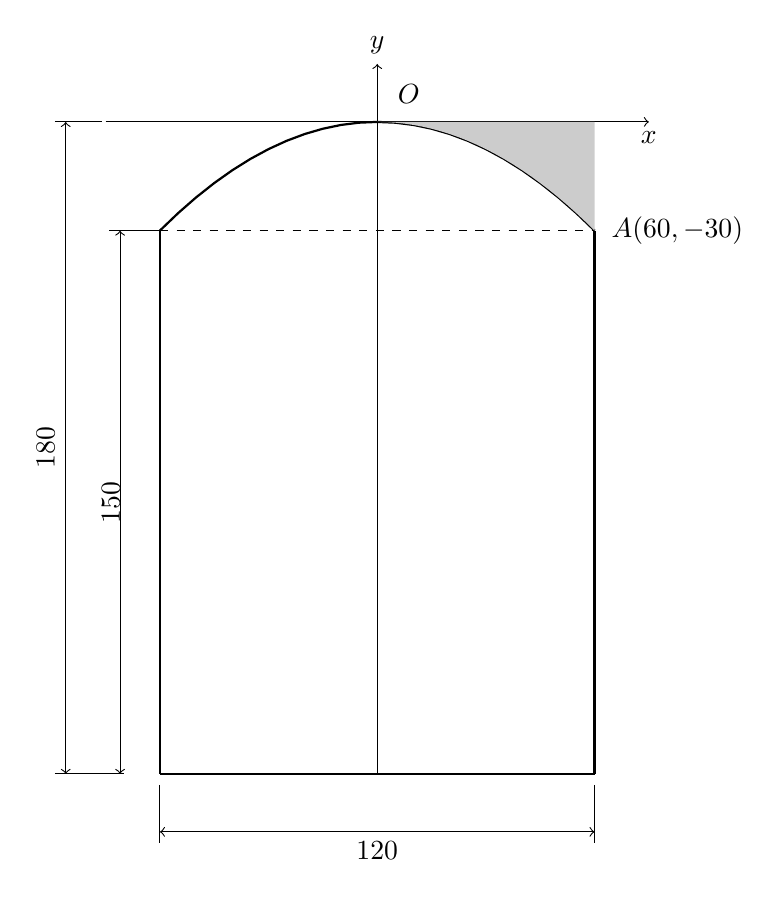
\begin{tikzpicture}[scale=0.46]
  \draw[->] (-7.5,0)--(7.5,0) node[below] {$x$};
  \draw[->] (0,-18)--(0,1.6) node[above] {$y$};
  \draw[thick] plot[domain=-6:6] (\x,{-\x*\x/12});
  \draw[thick] (-6,-3)--(-6,-18);
  \draw[thick] (6,-3)--(6,-18);
  \draw[thick] (-6,-18)--(6,-18);
  \draw[dashed] (-6,-3)--(6,-3);
  \fill[black!20] (0,0) -- plot[domain=0:6] (\x,{-\x*\x/12}) -- (6,0) -- cycle;
  \draw[<->] (-8.6,0)--(-8.6,-18);
  \draw (-8.9,0)--(-7.6,0);
  \draw (-8.9,-18)--(-7.0,-18);
  \node[rotate=90] at (-9.15,-9) {$180$};
  \draw[<->] (-7.1,-3)--(-7.1,-18);
  \draw (-7.4,-3)--(-6,-3);
  \node[rotate=90] at (-7.35,-10.5) {$150$};
  \draw (-6,-18.3)--(-6,-19.9);
  \draw (6,-18.3)--(6,-19.9);
  \draw[<->] (-6,-19.6)--(6,-19.6);
  \node[below] at (0,-19.6) {$120$};
  \node[above right] at (0.3,0.25) {$O$};
  \node[right] at (6.2,-3) {$A(60,-30)$};
\end{tikzpicture}
\end{center}
\nopagebreak[4]

\end{question}